\documentclass{standalone}
\usepackage{../preamble}

\begin{document}
\def\distance{150}
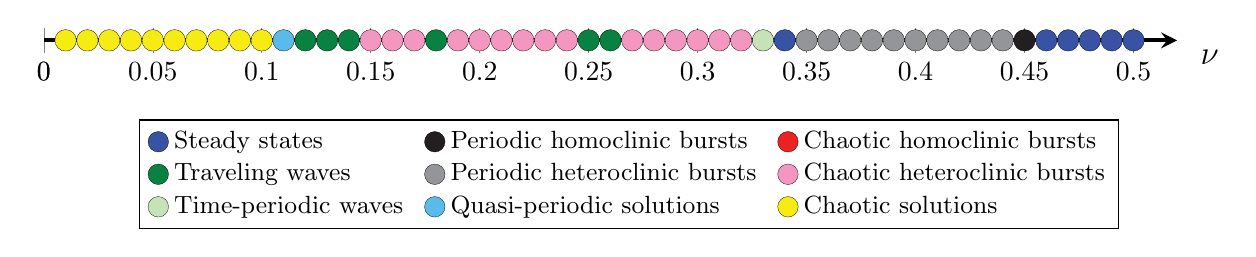
\begin{tikzpicture}[scale=2.1]
  \pgfplotsset{set layers}
  % colors
  \definecolor{myblue}{RGB}{57, 83, 164}
  \definecolor{myred}{RGB}{237, 32, 36}
  \definecolor{mydarkgreen}{RGB}{9, 129, 64}
  \definecolor{mylightgreen}{RGB}{198, 226, 183}
  \definecolor{mygray}{RGB}{147, 149, 152}
  \definecolor{myyellow}{RGB}{246, 235, 19}
  \definecolor{mypink}{RGB}{244, 151, 192}
  \definecolor{myblack}{RGB}{35, 31, 32}
  \definecolor{mycyan}{RGB}{89, 187, 234}
  \def\size{1.85pt}
  \begin{axis}[
      axis lines=middle,
      xmin=0, xmax=0.52,
      % remove y-axis
      axis y line=none,   % Hide y-axis
      %scale x-axis arrow
      x axis line style={-stealth,line width=1.5pt},
      % xtick=\empty, ytick=\empty,
      xlabel={$\nu$},
      xlabel style={below right, xshift=0.5em, font=\large},
      xtick={0, 0.05, ..., 1},
      % size of x and y ticks (do not use scientific notation)
      xticklabel style={scale=1, /pgf/number format/fixed},
      % include the 0 label
      extra x ticks={0,1},
      % legend (align text to the left)
      legend style={at={(0.246, 0.46)}, anchor=north, legend columns=3, fill=none, font=\small,transpose legend,/tikz/every even column/.append style={column sep=0.2cm},legend image post style={scale=2}},
      % text to the left of the legend
      legend cell align={left},
      % legend font scale
    ]



    % ALL THE CIRCLES ARE SYMMETRIC WITH RESPECT TO THE LINE y = x
    \addplot [only marks, mark=*, mark size=\size, draw=black, fill=myblue, ultra thin] coordinates
      {
        (0.5,0)
        (0.49,0)
        (0.48,0)
        (0.47,0)
        (0.46,0)
        (0.34,0)
      };
    \addplot [only marks, mark=*, mark size=\size, draw=black, fill=mydarkgreen, ultra thin] coordinates{
        (0.26,0)
        (0.25,0)
        (0.18,0)
        (0.14,0)
        (0.13,0)
        (0.12,0)
      };
    \addplot [only marks, mark=*, mark size=\size, draw=black, fill=mylightgreen, ultra thin] coordinates
      {
        (0.33,0)
      };
    \addplot [only marks, mark=*, mark size=\size, draw=black, fill=myblack, ultra thin] coordinates
      {
        (0.45,0)
      };
    \addplot [only marks, mark=*, mark size=\size, draw=black, fill=mygray, ultra thin] coordinates
      {
        (0.44,0)
        (0.43,0)
        (0.42,0)
        (0.41,0)
        (0.4,0)
        (0.39,0)
        (0.38,0)
        (0.37,0)
        (0.36,0)
        (0.35,0)
      };
    \addplot [only marks, mark=*, mark size=\size, draw=black, fill=mycyan, ultra thin] coordinates
      {
        (0.11,0)
      };
    \addplot [only marks, mark=*, mark size=\size, draw=black, fill=myred, ultra thin] coordinates
      {
        (2,0) % outside the domain but necessary to add it in the legend
      };
    \addplot [only marks, mark=*, mark size=\size, draw=black, fill=mypink, ultra thin] coordinates{
        (0.24,0)
        (0.27,0)
        (0.28,0)
        (0.21,0)
        (0.32,0)
        (0.31,0)
        (0.3,0)
        (0.29,0)
        (0.23,0)
        (0.22,0)
        (0.2,0)
        (0.19,0)
        (0.17,0)
        (0.16,0)
        (0.15,0)
      };
    \addplot [only marks, mark=*, mark size=\size, draw=black, fill=myyellow, ultra thin] coordinates
      {
        (0.1,0)
        (0.09,0)
        (0.08,0)
        (0.07,0)
        (0.06,0)
        (0.05,0)
        (0.04,0)
        (0.03,0)
        (0.02,0)
        (0.01,0)
      };
    % add legend
    \legend{Steady states,Traveling waves,Time-periodic waves,Periodic homoclinic bursts,Periodic heteroclinic bursts,Quasi-periodic solutions,Chaotic homoclinic bursts,Chaotic heteroclinic bursts,Chaotic solutions}
  \end{axis}
\end{tikzpicture}
\end{document}
